\documentclass[landscape,pdftex,headrule,footrule]{foils}
\usepackage{amsmath,amsthm,amsfonts,layout,verbatim}
\usepackage[pdftex]{graphicx}
\usepackage{url}
\usepackage{cfdlabfoils}
\usepackage{color}

\usepackage[
bookmarks=true,
colorlinks=true,
pdftex,
linkcolor=black,
filecolor=blue,
pagecolor=blue,
urlcolor=blue]
{hyperref}

\setlength\textheight{6.5in}
\setlength\topmargin{-2.5em}
\setlength\parindent{0pt}
\setlength\foilheadskip{.1in}

\newcommand{\bdoc}{\begin{document}}
\newcommand{\edoc}{\end{document}}
\newcommand{\ben}{\begin{enumerate}}
\newcommand{\een}{\end{enumerate}}
\newcommand{\binit}{\begin{itemize}}
\newcommand{\eit}{\end{itemize}}
\newcommand{\bdes}{\begin{description}}
\newcommand{\edes}{\end{description}}
\newcommand{\bc}{\begin{center}}
\newcommand{\ec}{\end{center}}
\newcommand{\bflt}{\begin{flushleft}}
\newcommand{\eflt}{\end{flushleft}}
\newcommand{\bfrt}{\begin{flushright}}
\newcommand{\efrt}{\end{flushright}}
\newcommand{\be}{\begin{equation}}
\newcommand{\ee}{\end{equation}}
\newcommand{\bes}{\begin{displaymath}}
\newcommand{\ees}{\end{displaymath}}
\newcommand{\ba}{\begin{array}}
\newcommand{\ea}{\end{array}}
\newcommand{\bea}{\begin{eqnarray}}
\newcommand{\eea}{\end{eqnarray}}
\newcommand{\beas}{\begin{eqnarray*}}
\newcommand{\eeas}{\end{eqnarray*}}
\newcommand{\np}{\newpage}
\newcommand{\bsni}{\bigskip \noindent}
\newcommand{\nn}{\nonumber}
\newcommand{\ds}{\displaystyle}
\newcommand{\ts}{\textstyle}
\newcommand{\sstyle}{\scriptstyle}
\newcommand{\ssstyle}{\scriptscriptstyle}
%
\newcommand{\Dt}{\mbox{${\Delta t}$}}
\newcommand{\Dx}{\mbox{${\Delta x}$}}
%
\newcommand{\bfa}{\mbox{\boldmath $a$}}
\newcommand{\bfb}{\mbox{\boldmath $b$}}
\newcommand{\bfc}{\mbox{\boldmath $c$}}
\newcommand{\bfd}{\mbox{\boldmath $d$}}
\newcommand{\bfe}{\mbox{\boldmath $e$}}
\newcommand{\bff}{\mbox{\boldmath $f$}}
\newcommand{\bfg}{\mbox{\boldmath $g$}}
\newcommand{\bfh}{\mbox{\boldmath $h$}}
\newcommand{\bfi}{\mbox{\boldmath $i$}}
\newcommand{\bfj}{\mbox{\boldmath $j$}}
\newcommand{\bfk}{\mbox{\boldmath $k$}}
\newcommand{\bfl}{\mbox{\boldmath $l$}}
\newcommand{\bfm}{\mbox{\boldmath $m$}}
\newcommand{\bfn}{\mbox{\boldmath $n$}}
\newcommand{\bfo}{\mbox{\boldmath $o$}}
\newcommand{\bfp}{\mbox{\boldmath $p$}}
\newcommand{\bfq}{\mbox{\boldmath $q$}}
\newcommand{\bfr}{\mbox{\boldmath $r$}}
\newcommand{\bfs}{\mbox{\boldmath $s$}}
\newcommand{\bft}{\mbox{\boldmath $t$}}
\newcommand{\bfu}{\mbox{\boldmath $u$}}
\newcommand{\bfv}{\mbox{\boldmath $v$}}
\newcommand{\bfw}{\mbox{\boldmath $w$}}
\newcommand{\bfx}{\mbox{\boldmath $x$}}
\newcommand{\bfy}{\mbox{\boldmath $y$}}
\newcommand{\bfz}{\mbox{\boldmath $z$}}
%
\newcommand{\bfA}{\mbox{\boldmath $A$}}
\newcommand{\bfB}{\mbox{\boldmath $B$}}
\newcommand{\bfC}{\mbox{\boldmath $C$}}
\newcommand{\bfD}{\mbox{\boldmath $D$}}
\newcommand{\bfE}{\mbox{\boldmath $E$}}
\newcommand{\bfF}{\mbox{\boldmath $F$}}
\newcommand{\bfG}{\mbox{\boldmath $G$}}
\newcommand{\bfH}{\mbox{\boldmath $H$}}
\newcommand{\bfI}{\mbox{\boldmath $I$}}
\newcommand{\bfJ}{\mbox{\boldmath $J$}}
\newcommand{\bfK}{\mbox{\boldmath $K$}}
\newcommand{\bfL}{\mbox{\boldmath $L$}}
\newcommand{\bfM}{\mbox{\boldmath $M$}}
\newcommand{\bfN}{\mbox{\boldmath $N$}}
\newcommand{\bfO}{\mbox{\boldmath $O$}}
\newcommand{\bfP}{\mbox{\boldmath $P$}}
\newcommand{\bfQ}{\mbox{\boldmath $Q$}}
\newcommand{\bfR}{\mbox{\boldmath $R$}}
\newcommand{\bfS}{\mbox{\boldmath $S$}}
\newcommand{\bfT}{\mbox{\boldmath $T$}}
\newcommand{\bfU}{\mbox{\boldmath $U$}}
\newcommand{\bfV}{\mbox{\boldmath $V$}}
\newcommand{\bfW}{\mbox{\boldmath $W$}}
\newcommand{\bfX}{\mbox{\boldmath $X$}}
\newcommand{\bfY}{\mbox{\boldmath $Y$}}
\newcommand{\bfZ}{\mbox{\boldmath $Z$}}
%
\newcommand{\alp}{{\alpha}}
\newcommand{\bet}{{\beta}}
\newcommand{\gam}{{\gamma}}
\newcommand{\del}{{\delta}}
\newcommand{\eps}{{\epsilon}}
\newcommand{\vareps}{{\varepsilon}}
\newcommand{\zet}{{\zeta}}
\newcommand{\thet}{{\theta}}
\newcommand{\varthet}{\vartheta}
\newcommand{\iot}{{\iota}}
\newcommand{\kap}{{\kappa}}
\newcommand{\lam}{{\lambda}}
\newcommand{\sig}{{\sigma}}
\newcommand{\ups}{{\upsilon}}
\newcommand{\ome}{{\omega}}
%
\newcommand{\Gam}{{\Gamma}}
\newcommand{\Del}{{\Delta}}
\newcommand{\Thet}{{\Theta}}
\newcommand{\Lam}{{\Lambda}}
\newcommand{\Sig}{{\Sigma}}
\newcommand{\Ups}{{\Upsilon}}
\newcommand{\Ome}{{\Omega}}
%
\newcommand{\bfalp}{\mbox{\boldmath $\alpha$}}
\newcommand{\bfbet}{\mbox{\boldmath $\beta$}}
\newcommand{\bfgam}{\mbox{\boldmath $\gamma$}}
\newcommand{\bfdel}{\mbox{\boldmath $\delta$}}
\newcommand{\bfeps}{\mbox{\boldmath $\epsilon$}}
\newcommand{\bfvareps}{\mbox{\boldmath $\varepsilon$}}
\newcommand{\bfzet}{\mbox{\boldmath $\zeta$}}
\newcommand{\bfeta}{\mbox{\boldmath $\eta$}}
\newcommand{\bfthet}{\mbox{\boldmath $\theta$}}
\newcommand{\bfiot}{\mbox{\boldmath $\iota$}}
\newcommand{\bfkap}{\mbox{\boldmath $\kappa$}}
\newcommand{\bflam}{\mbox{\boldmath $\lambda$}}
\newcommand{\bfmu}{\mbox{\boldmath $\mu$}}
\newcommand{\bfnu}{\mbox{\boldmath $\nu$}}
\newcommand{\bfxi}{\mbox{\boldmath $\xi$}}
\newcommand{\bfpi}{\mbox{\boldmath $\pi$}}
\newcommand{\bfrho}{\mbox{\boldmath $\rho$}}
\newcommand{\bfsig}{\mbox{\boldmath $\sigma$}}
\newcommand{\bftau}{\mbox{\boldmath $\tau$}}
\newcommand{\bfups}{\mbox{\boldmath $\upsilon$}}
\newcommand{\bfphi}{\mbox{\boldmath $\phi$}}
\newcommand{\bfchi}{\mbox{\boldmath $\chi$}}
\newcommand{\bfpsi}{\mbox{\boldmath $\psi$}}
\newcommand{\bfome}{\mbox{\boldmath $\omega$}}
%
\newcommand{\bfGam}{\mbox{\boldmath $\Gamma$}}
\newcommand{\bfDel}{\mbox{\boldmath $\Delta$}}
\newcommand{\bfThet}{\mbox{\boldmath $\Theta$}}
\newcommand{\bfLam}{\mbox{\boldmath $\Lambda$}}
\newcommand{\bfXi}{\mbox{\boldmath $\Xi$}}
\newcommand{\bfPi}{\mbox{\boldmath $\Pi$}}
\newcommand{\bfSig}{\mbox{\boldmath $\Sigma$}}
\newcommand{\bfUps}{\mbox{\boldmath $\Upsilon$}}
\newcommand{\bfPhi}{\mbox{\boldmath $\Phi$}}
\newcommand{\bfPsi}{\mbox{\boldmath $\Psi$}}
\newcommand{\bfOme}{\mbox{\boldmath $\Omega$}}
%
\newcommand{\ptl}{{\partial}}
\newcommand{\nab}{{\nabla}}
%
\newcommand{\bfptl}{\mbox{\boldmath $\partial$}}
\newcommand{\bfnab}{\mbox{\boldmath $\nabla$}}
\newcommand{\bfinfty}{\mbox{\boldmath $\infty$}}
\newcommand{\bfto}{\mbox{\boldmath $\to$}}
\newcommand{\bfimath}{\mbox{\boldmath $\imath$}}
\newcommand{\bfjmath}{\mbox{\boldmath $\jmath$}}
\newcommand{\bfsum}{\mbox{\boldmath $\sum$}}
%
\newcommand{\calA}{\mbox{${\cal A}$}}
\newcommand{\calB}{\mbox{${\cal B}$}}
\newcommand{\calC}{\mbox{${\cal C}$}}
\newcommand{\calD}{\mbox{${\cal D}$}}
\newcommand{\calE}{\mbox{${\cal E}$}}
\newcommand{\calF}{\mbox{${\cal F}$}}
\newcommand{\calG}{\mbox{${\cal G}$}}
\newcommand{\calH}{\mbox{${\cal H}$}}
\newcommand{\calI}{\mbox{${\cal I}$}}
\newcommand{\calJ}{\mbox{${\cal J}$}}
\newcommand{\calK}{\mbox{${\cal K}$}}
\newcommand{\calL}{\mbox{${\cal L}$}}
\newcommand{\calM}{\mbox{${\cal M}$}}
\newcommand{\calN}{\mbox{${\cal N}$}}
\newcommand{\calO}{\mbox{${\cal O}$}}
\newcommand{\calP}{\mbox{${\cal P}$}}
\newcommand{\calQ}{\mbox{${\cal Q}$}}
\newcommand{\calR}{\mbox{${\cal R}$}}
\newcommand{\calS}{\mbox{${\cal S}$}}
\newcommand{\calT}{\mbox{${\cal T}$}}
\newcommand{\calU}{\mbox{${\cal U}$}}
\newcommand{\calV}{\mbox{${\cal V}$}}
\newcommand{\calW}{\mbox{${\cal W}$}}
\newcommand{\calX}{\mbox{${\cal X}$}}
\newcommand{\calY}{\mbox{${\cal Y}$}}
\newcommand{\calZ}{\mbox{${\cal Z}$}}
%
\newcommand{\degrees}{\mbox{$^\circ$}}
\newcommand{\pdv}[2]{\frac{\partial{#1}}{\partial{#2}}}
\newcommand{\dv}[2]{\frac{d{#1}}{d{#2}}}
\newcommand{\intgl}[2]{\ds \int^{#1}_{#2}}
\newcommand{\sums}[2]{\ds \sum^{#1}_{#2}}
\newcommand{\dsfrac}[2]{\ds \frac{#1}{#2}}
\newcommand{\tsfrac}[2]{\ts \frac{#1}{#2}}
\newcommand{\ldb}{\ [\![\ }
\newcommand{\rdb}{\ ]\!]\ } 
\newcommand{\ia}{\int\!\!\!\int\limits_{\!\!\!\!\rm Area}}
\newcommand{\RR}{R\!\!\!\!R}
\newcommand{\fR}{\mbox{I}\!\mbox{R}}
\newcommand{\fC}{\mbox{I}\!\!\!\!\!\;\mbox{C}}
\newcommand{\vbar}{\vee \!\!\!\!\!\! -}
\newcommand{\wh}{\widehat}



\newcommand{\libMesh}{\href{http://libmesh.sourceforge.net}{\texttt{libMesh\ }}}

\hyperbaseurl{/home/benkirk/phd/dissertation/progress}

\title{Progress Report}
\author{\vspace{1in} \\ Benjamin S. Kirk}


\MyLogo{\href{http://cfdlab.ae.utexas.edu/}{CFDLab}, The University of Texas at Austin}


%\rightheader{\includegraphics[height=.8in]{figures/word3}}
%\leftheader{\includegraphics[height=.8in]{figures/utlogo}}

\begin{document}
%\layout
\maketitle


%%%%%%%%%%%%%%%%%%%%%%%%%%%%%%%%%%%%%%%%%%%%%%%%%%%%%%%%%%%%%%%%%%%%%%%%%%%%%%%
\begin{foil}{Outline}
  \begin{itemize}
    \tightlist
    \item Motivation
    \item Anticipated contributions
    \item Monotonicity \& positivity-preserving algorithms
    \item Nested Grids 
      \begin{itemize}
	\item Uniform meshes
	\item Adaptive meshes
      \end{itemize}
    \item Subgrid strategies
    \item Adaptive refinement
      \begin{itemize}
	\item Data structures
	\item Parallel issues
      \end{itemize}
    \item Applications \& phenomenological studies
    \item Roadmap
  \end{itemize}
\end{foil}


%%%%%%%%%%%%%%%%%%%%%%%%%%%%%%%%%%%%%%%%%%%%%%%%%%%%%%%%%%%%%%%%%%%%%%%%%%%%%%%
\begin{foil}{Motivation}
  \begin{itemize}
    \tightlist
    \item Persistent problems in CFD
      \begin{itemize}
	\item Accuracy and Stability
	\item Stabilization
	\item Multiscale phenomenon
      \end{itemize}
    \item Advanced numerical techniques
      \begin{itemize}
        \item Monotonicity
	\item Adaptivity
	\item Parallel Computing
      \end{itemize}
    \item These ideas must all be tied together to \emph{efficiently} simulate current problems of interest 
  \end{itemize}
\end{foil}


%%%%%%%%%%%%%%%%%%%%%%%%%%%%%%%%%%%%%%%%%%%%%%%%%%%%%%%%%%%%%%%%%%%%%%%%%%%%%%%
\begin{foil}{Anticipated Contributions}
  \begin{itemize}
    \tightlist
    \item Major Contributions
      \begin{itemize}
	\item Monotonicity/positivity preserving algorithms
	\item Nested Grid Approaches
	\item Subgrid Strategies for solution enhancement and stabilization
	\item Applications \& phenomenological studies
      \end{itemize}
    \item Other Contributions
      \begin{itemize}
	\item Adaptive mesh refinement research
	\item Parallel data structures
      \end{itemize}
  \end{itemize}
\end{foil}


%%%%%%%%%%%%%%%%%%%%%%%%%%%%%%%%%%%%%%%%%%%%%%%%%%%%%%%%%%%%%%%%%%%%%%%%%%%%%%%
\begin{foil}{Monotonicity -- Problem Description}
  \stepwise*{
    \FirstOnly{}{
      \begin{itemize}
	\tightlist
        \item Single-species general reactive transport:
	  \begin{equation}
            \frac{\partial C}{\partial t} + \nabla \cdot (\bfu C - D \nabla C)  = R(C)
            \label{eqn:cdr}
	  \end{equation}
	\item $R(C)$ describes a broad range of physical processes
	  \begin{itemize}
            \item Radioactive decay ($R(C) = -\mu C$)
            \item Population growth ($R(C) = \mu_1 C - \mu_2 C^2$)
            \item Biodegredation ($\frac{\mu C}{K + C}$)
            \item Others\ldots
	  \end{itemize}
      \end{itemize}
    }
    \FirstOnly{}{
      \begin{itemize}
        \item The transport variable $C$ defines the concentration field
	\item Physically, the concentration is \emph{nonnegative}.  Many reaction models assume this.
	\item Negative concentrations can lead to mass-imbalance and convergence problems
	\item Typically, the concentration field may be ``clipped'' when computing reactions
      \end{itemize}
    }
  }
\end{foil}
 
 
 
%%%%%%%%%%%%%%%%%%%%%%%%%%%%%%%%%%%%%%%%%%%%%%%%%%%%%%%%%%%%%%%%%%%%%%%%%%%%%%
\begin{foil}{Possible Solution}
  \begin{itemize}
    \item Construct a monotone discretization that will not admit negative concentrations
      \begin{itemize}
        \item Flux-limited, finite difference discretization is used in 1D to
              construct a discrete system with the desired properties.
        \item 1D theory has been applied 2D on uniform grids.
        \item Can be directly applied to finite elements on
              structured grids.
      \end{itemize}
    \item Attempt to extend the 1D theory presented by MacKinnon and Carey to 2D.
  \end{itemize}
\end{foil}

                                                                                
                                                                                
%%%%%%%%%%%%%%%%%%%%%%%%%%%%%%%%%%%%%%%%%%%%%%%%%%%%%%%
\begin{foil}{Flux-Limited FD Scheme}
  \begin{equation}
    \frac{\partial C}{\partial t} + \nabla \cdot (\bfu C - D \nabla C)  = \left[R_1(C) - R_2(C)\right] C
    \nonumber
  \end{equation}
  Using standard finite differencing:
  \begin{eqnarray}
    \nonumber
    \left(\frac{1}{\Delta t}\bfI + \theta (\bfD + \bfU(\lambda)) + \alpha_1 \bfI R_1(C) - \alpha_2 \bfI R_2(C) \right) \bfc^{n+1} = \\ \nonumber
    \left(\frac{1}{\Delta t}\bfI - (1-\theta) (\bfD + \bfU(\lambda)) - (1-\alpha_1) \bfI R_1(C^n) + (1-\alpha_2) \bfI R_2(C^n) \right) \bfc^{n}
  \end{eqnarray}
  where $\bfD$ and $\bfU(\lambda)$ are the discrete diffusion and convection operators, $\lambda = \lambda(C)$ is a flux-limiter,
  and $\theta, \alpha_1, \alpha_2 \in [0,1]$ govern the behavior of the scheme.
                                                                                
\end{foil}


                                                                                
%%%%%%%%%%%%%%%%%%%%%%%%%%%%%%%%%%%%%%%%%%%%%%%%%%%%%%%
\begin{foil}{Flux-Limited FD Scheme}
  \begin{itemize}
    \item The flux limiter $\lambda$ is chosen so that the resulting linear
          system has three important properties:
    \begin{enumerate}
      \item Nonnegative stiffness matrix $\bfK: K_{ij} \ge 0$
      \item Nonnegative right-hand-side  $\bff: f_i \ge 0$
      \item Strict diagonal dominance: $K_{ii} > \sum K_{ij}, \; i \ne j$
    \end{enumerate}
  \item Leads to a nonlinear system since $\lambda = \lambda(C)$
  \item For certain $\theta, \alpha_1, \alpha_2$ leads to a \emph{lower bound}
        on the timestep $\Delta t$
  \end{itemize}
\end{foil}



%%%%%%%%%%%%%%%%%%%%%%%%%%%%%%%%%%%%%%%%%%%%%%%%%%%%%%%
\begin{foil}{Numerical Experiments}
  \stepwise*{
    \FirstOnly{}{
      \vspace{-.4in}
      \zerolistvertdimens  
      \begin{minipage}[h]{.5\textwidth}
	\begin{figure}[h]
	  \begin{center}
            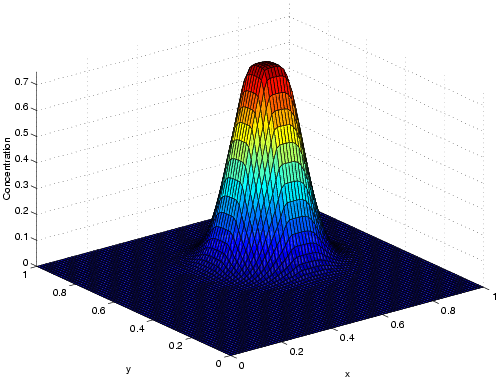
\includegraphics[width=\textwidth]{figures/case5b_1_fine}
	  \end{center}
	\end{figure}
      \end{minipage}
      \begin{minipage}[h]{.5\textwidth}
	\begin{figure}[h]
	  \begin{center}
            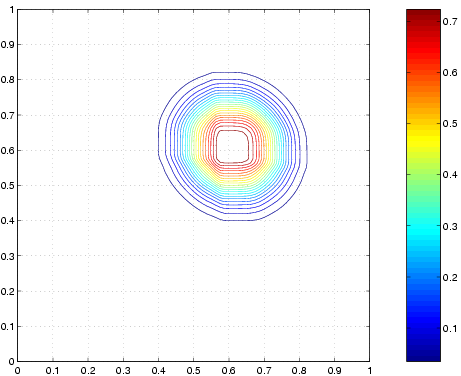
\includegraphics[width=\textwidth]{figures/case5b_2_fine}
	  \end{center}
	\end{figure}
      \end{minipage}
      
      \vspace{.2in}
      \begin{itemize}
	\tightlist
        \item $R(C) = 0.4\left[C - C^2\right]$, $\theta = 0$, $\alpha_1 = \alpha_2 = 1$
	\item Profile exhibits some mesh aligned ``squaring''
      \end{itemize}
    }
    \FirstOnly{}{
      \vspace{-.4in}
      \zerolistvertdimens
      \begin{minipage}[h]{.5\textwidth}
	\begin{figure}[h]
	  \begin{center}
            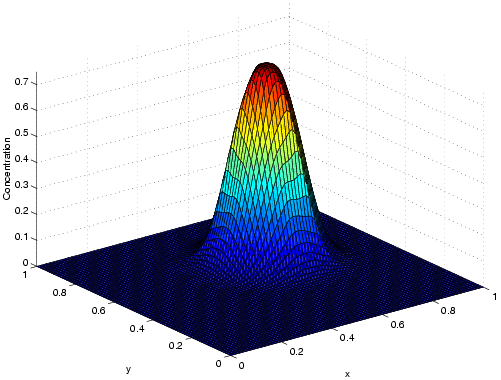
\includegraphics[width=\textwidth]{figures/case6a_1_fine}
	  \end{center}
	\end{figure}
      \end{minipage}
      \begin{minipage}[h]{.5\textwidth}
	\begin{figure}[h]
	  \begin{center}
            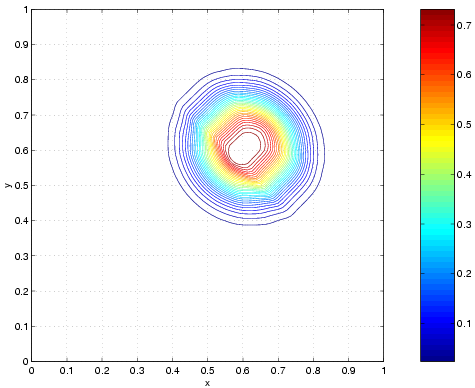
\includegraphics[width=\textwidth]{figures/case6a_2_fine}
	  \end{center}
	\end{figure}
      \end{minipage}
      
      \vspace{.2in}
      \begin{itemize}
	\tightlist
        \item $R(C) = 0.4\left[C - C^2\right]$, $\theta = 0$, $\alpha_1 = \alpha_2 = 1$
	\item Split stencil: $\frac{2}{3}$ standard + $\frac{1}{3}$ rotated
      \end{itemize}
    }
  }
\end{foil}
                                                                                
                                                                                
                                                                                
                                                                                
%%%%%%%%%%%%%%%%%%%%%%%%%%%%%%%%%%%%%%%%%%%%%%%%%%%%%%%
\begin{foil}{Discussion - FD Scheme}
  \begin{itemize}
    \item Naive extension of the 1D theory yields distorted results
          (this behavior is common among TVD schemes).
    \item Not clear that using a rotated stencil improves performance.
    \item Matrix structure seems preserved in 2D, solution remains positive.
    \item Requires a ``lumped'' mass matrix, which admits phase errors.
  \end{itemize}
  \vspace{.25in}
  \emph{* Paper in progress detailing 2D extension}
  
  \emph{* Presented at the 2003  SIAM Conference on Mathematical and Computational Issues in the Geosciences}
\end{foil}
                                                                                
                                                                                
                                                                                
                                                                                
%%%%%%%%%%%%%%%%%%%%%%%%%%%%%%%%%%%%%%%%%%%%%%%%%%%%%%%
\begin{foil}{Nested Grids}
  \begin{itemize}
    \item Cascadic multigrid for nonsymmetric, nonlinear problems
      \begin{itemize}
	\item Can be applied to existing codes via restart
      \end{itemize}
    \item Adaptive mesh refinement extensions
      \begin{itemize}
	\item Produces quality adaptive grids without \emph{a posteriori} error indicators
      \end{itemize}
  \end{itemize}
\end{foil}



%%%%%%%%%%%%%%%%%%%%%%%%%%%%%%%%%%%%%%%%%%%%%%%%%%%%%%%%%%%%%%%%%%%%%%%%%%%%%%%
\begin{foil}[-.25in]{Nested Refinement -- Algorithm}
  \begin{minipage}[h]{.3\textwidth}
    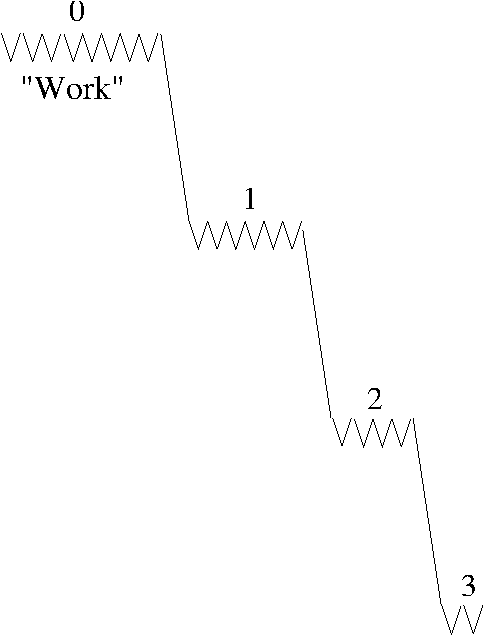
\includegraphics[width=\textwidth]{figures/cmg}
  \end{minipage}
  \begin{minipage}[h]{.7\textwidth}
    \begin{tabular}{lp{4in}}
      $j=0$ : &  $u_0^h \equiv u_j^*$ \\
      &  precise solution on the coarse grid\\[2.9ex]
      %
      $j=1,\ldots, L$ : & $u_j^0={\cal P}_j u_{j-1}^*$\\
      & interpolation to the finer grid\\[2.9ex]
      %
      & $u_j^*={\cal I}_j(m_j) u_{j}^0$\\
      & iterative solution of problems
      on successively finer grids \\[2.9ex]
    \end{tabular}
  \end{minipage}
  
  \vspace{1in}
  
  \centerline{\noindent Stopping criterion: $\| u - u^h_L\|_a \approx \|u^h_L - u_L^{*}\|_a$}
\end{foil}



%%%%%%%%%%%%%%%%%%%%%%%%%%%%%%%%%%%%%%%%%%%%%%%%%%%%%%%%%%%%
\begin{foil}{Cascadic MG: Estimates}
  
  $\bullet$ Shaidurov (1996), Deuflhard, Bornemann (1996)
 
  \small
  \begin{tabular}{cl}
    Approximation & \hspace*{3.5mm} $\| u - u_j^h \|_a  \le  c h_j \| f \|_0$\\[1.0ex]
    assumptions:  & $\| u_j^h - u_{j-1}^h \|_0  \le  c h_j \| u_j^h
                   - u_{j-1}^h\|_a \quad 1 \le j \le L$ \\[3.0ex]
    %
    Smoothing     & $\| S_j(m_j) v_j^h \|_a  \le
                    c \frac{h_j^{-1}}{m_j^\gamma} \| v_j^h\|_0$ \\[1.0ex]
    assumptions:  & $\| S_j(m_j) v_j^h \|_a  \le \| v_j^h \|_a \qquad \qquad
                    \forall v_j^h \in V_j$\\[3.0ex]
  \end{tabular}\\
  where $S_j$ is the error propagation operator. Then
  $$
   \| u_L^h - u_L^* \|_a \le c \sum\limits_{j=1}^L \frac{1}{m_j^\gamma}
   \| u_j^h - u_{j-1}^h \|_a \le
   c \left( \sum\limits_{j=1}^L \frac{h_j}{m_j^\gamma} \right) \| f \|_0.
  $$
 
   \noindent Note:  $\gamma = 1$ for CG \newline
   \hphantom{Note:} $\gamma = 1/2$ for Jacobi, SSOR, symmetric GS.
   \normalsize
   
\end{foil}



%%%%%%%%%%%%%%%%%%%%%%%%%%%%%%%%%%%%%%%%%%%%%%%%%%%%%%%%%%%%%%%%%%%%%%%%%%%%%%%
\begin{foil}[-.5in]{Numerical Experiments}
  \vspace{-1in}
  \begin{minipage}[h]{.5\textwidth}
    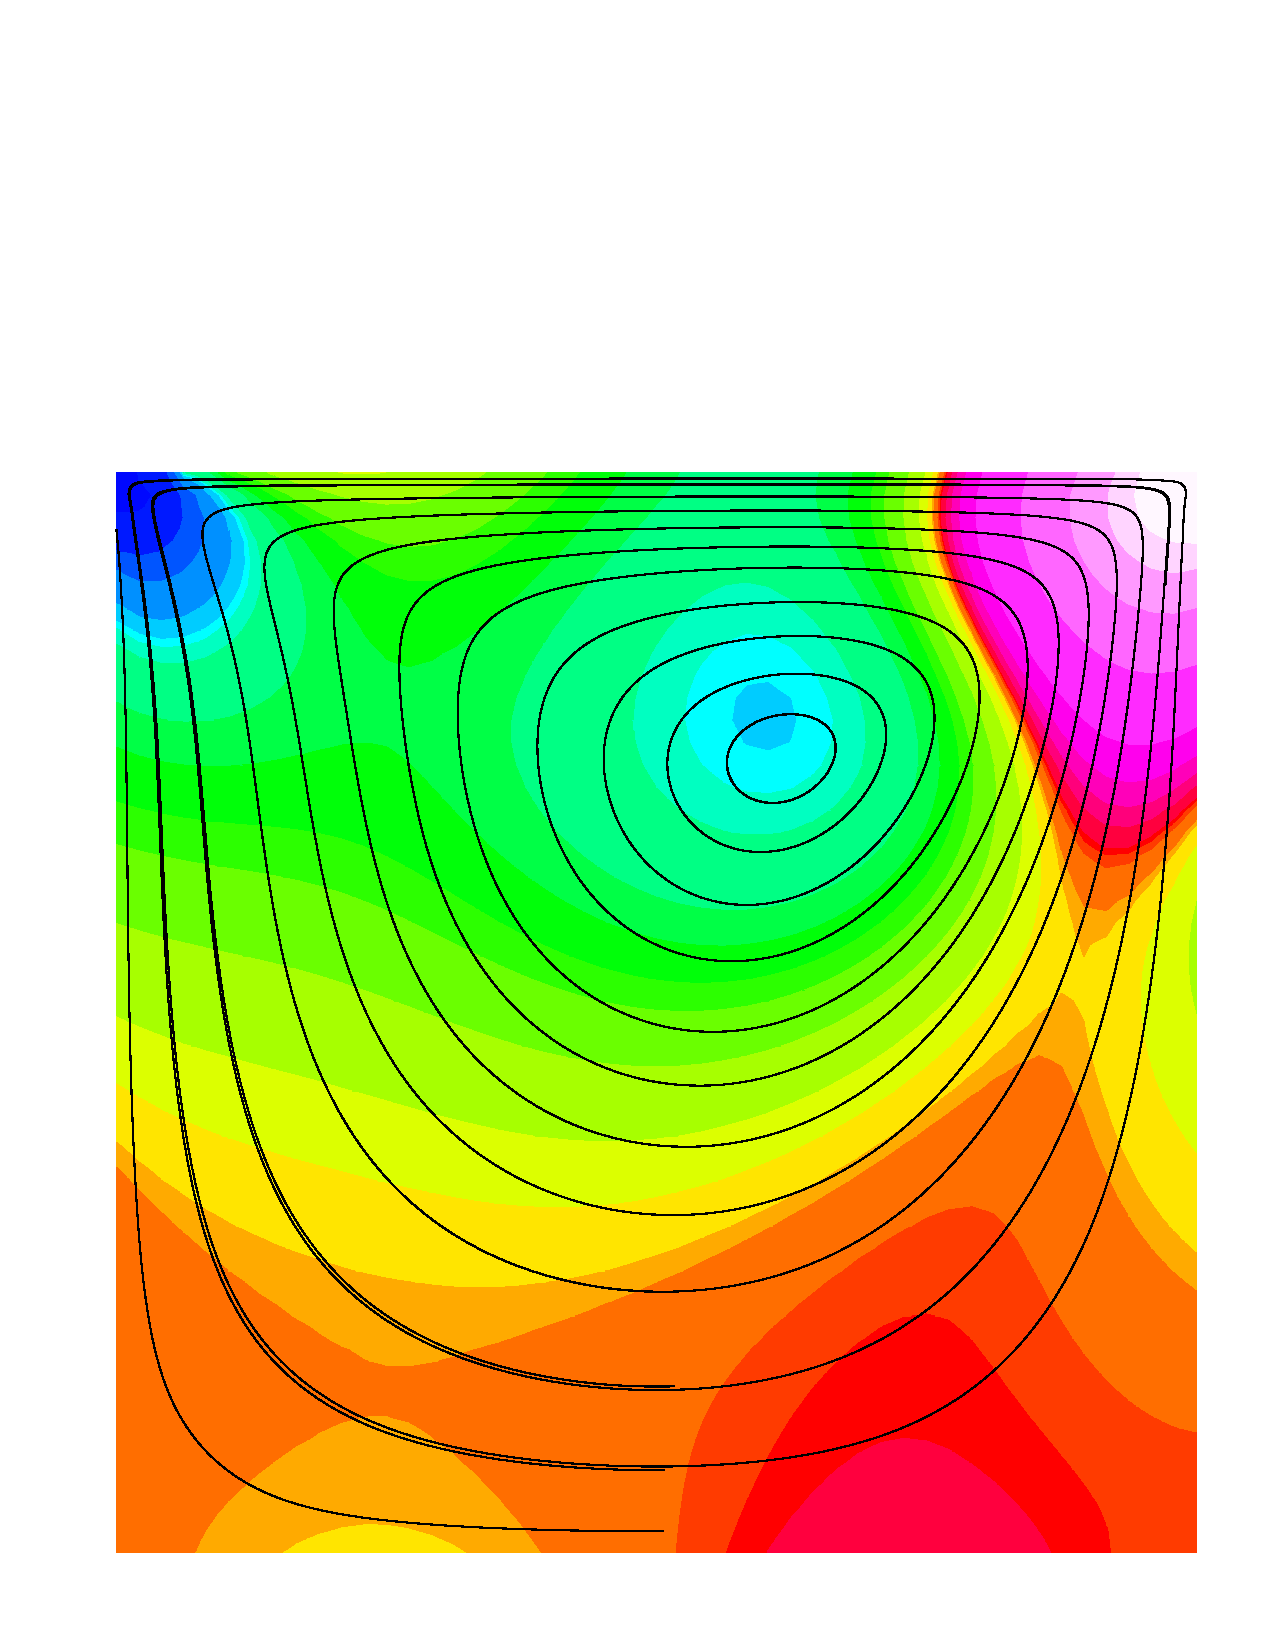
\includegraphics[width=\textwidth]{figures/flowfield-2D}
  \end{minipage}
  \begin{minipage}[h]{.5\textwidth}
    \textbf{2D Driven Cavity}
    \begin{itemize}
      \item Jacobi--preconditioned
      \item GMRES-50, BCG, \& BCG--Stab solvers
      \item Convergence histories examined
    \end{itemize}
  \end{minipage}
\end{foil}



%%%%%%%%%%%%%%%%%%%%%%%%%%%%%%%%%%%%%%%%%%%%%%%%%%%%%%%%%%%%
\begin{foil}[-.3in]{Numerical Experiments}
  
  Convergence details (total iterations per mesh)
  
  \tiny
  \begin{centering}
    

    \begin{tabular}{l r}

      
    
    BCG: &
    \begin{tabular}{|l|r|r|r|r|} \hline
                   & 6x6 & 12x12 & 24x24 & 48x48 \\ \hline
           CMG     & 448 &  952  & 1767  & 6875  \\ \hline
         No MG     & 448 &  1157 & 2940  & 11124 \\ \hline
       Work Factor & 1   &  0.82 & 0.60  & 0.62  \\ \hline
    \end{tabular}

    \\
     & \\
     & \\
    \\
    
    BCG--Stab: &
    \begin{tabular}{|l|r|r|r|r|} \hline
                   & 6x6 & 12x12 & 24x24 & 48x48 \\ \hline
           CMG     & 513 & 757   & 1663  & 2513  \\ \hline
         No MG     & 513 & 1056  & 2571  & 6154  \\ \hline
       Work Factor & 1   & 0.72  & 0.65  & 0.41  \\ \hline
    \end{tabular}

    \\
     & \\
     & \\
    \\

    
 
    GMRES--50: &
    \begin{tabular}{|l|r|r|r|r|} \hline
                   & 6x6 & 12x12 & 24x24 & 48x48 \\ \hline
           CMG     & 681 & 1261  & 2442  & 5696  \\ \hline
         No MG     & 681 & 1657  & 4719  & 17678 \\ \hline
       Work Factor & 1   & 0.76  & 0.52  & 0.32  \\ \hline
    \end{tabular}
    \\
    \end{tabular}
\end{centering}
 
\normalsize
 
$\bullet$ Most benefit with GMRES, least with BCG

\emph{* Results Published in IJCFD Vol. 17, August 2003}
\end{foil}



%%%%%%%%%%%%%%%%%%%%%%%%%%%%%%%%%%%%%%%%%%%%%%%%%%%%%%%%%%%%
\begin{foil}[-.5in]{Numerical Experiments -- Linear Solver Performance}
  \centerline{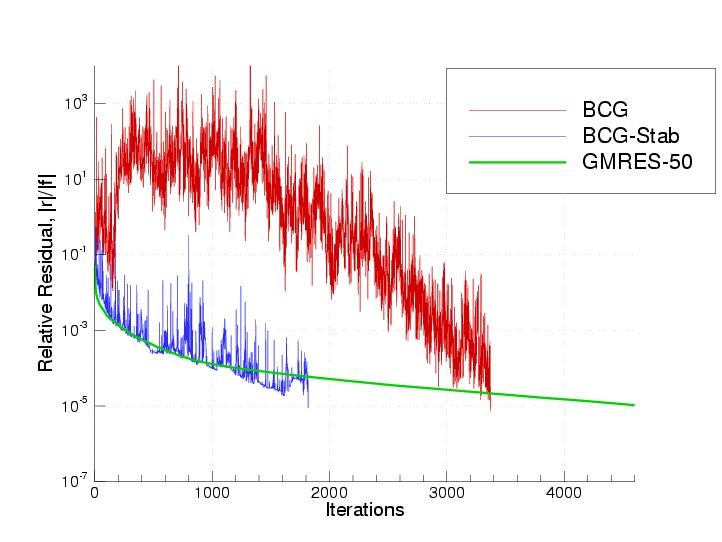
\includegraphics[width=.9\textwidth]{figures/history}}
\end{foil}



%%%%%%%%%%%%%%%%%%%%%%%%%%%%%%%%%%%%%%%%%%%%%%%%%%%%%%%%%%%%%%%%%%%%%%%%%%%%%%%
\begin{foil}[-.25in]{Nested Refinement}
  \begin{itemize}
    \item Motivated by one--way multigrid techniques for elliptic problems
    \item The mesh is uniformly refined at each refinement step
    \item The error is computed as $e_f=\|u_{f} - {\cal P}_f^c (u_{c}) \|$
    \item Cells may be unrefined in regions where the error is small
      \vspace{.25in}
      \centerline{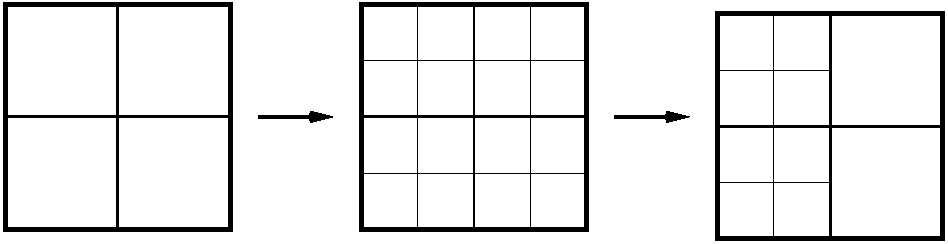
\includegraphics[height=.2\textheight]{figures/refine2}}
    \item Hanging nodes are constrained to ensure continuity
  \end{itemize}
\end{foil}



%%%%%%%%%%%%%%%%%%%%%%%%%%%%%%%%%%%%%%%%%%%%%%%%%%%%%%%%%%%%%%%%%%%%%%%%%%%%%%%
\begin{foil}{Natural Convection}
  \stepwise*{
    \FirstOnly{}{
      \begin{minipage}[h]{.5\textwidth}
        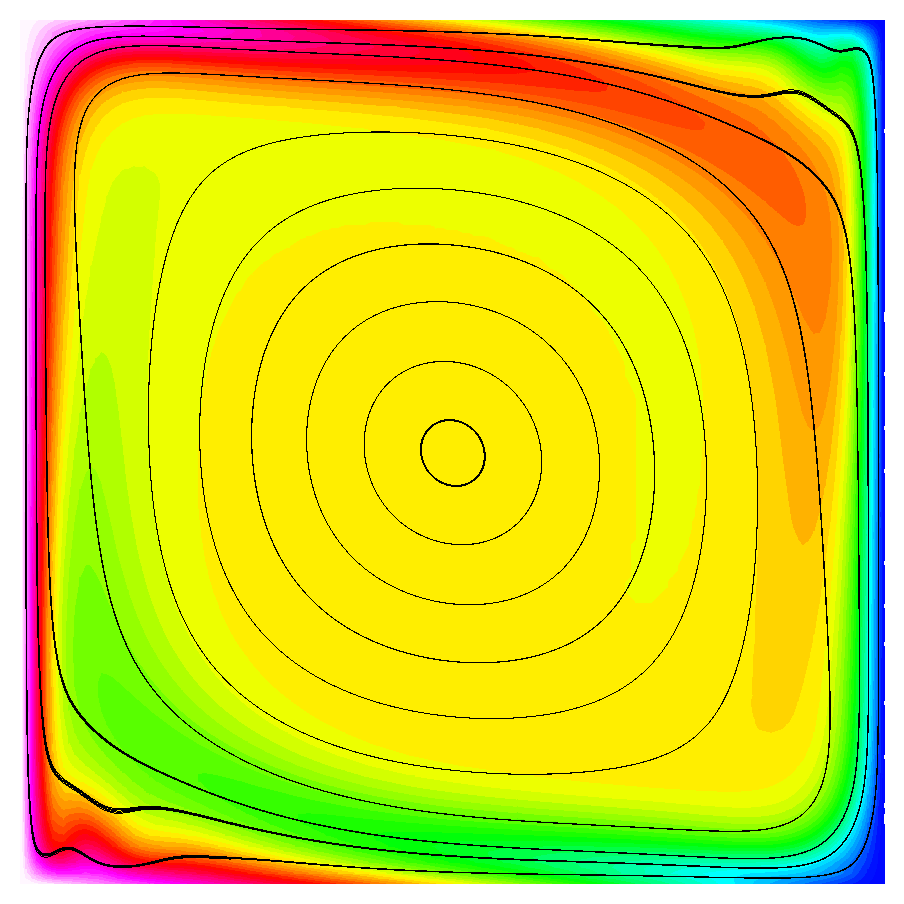
\includegraphics[width=\textwidth]{figures/lid}
      \end{minipage}
      \begin{minipage}[h]{.5\textwidth}
        \begin{itemize}
          \item Natural convection induced by a horizontal temperature gradient in a .1272m square
          \item Air, $Ra=10^7$
          \item Solved time--dependent to steady--state
          \item Want to capture transients on coarse mesh
          \item Nested iteration reduced solution time by an order of magnitude
        \end{itemize}
      \end{minipage}
    }
   
    \FirstOnly{}{
      \vspace{-1in}
      \begin{center}
        \begin{tabular}{l c c r}
	  Start & & & \\
          
\includegraphics[height=.22\textheight]{figures/grid0} & & & \\
	  & 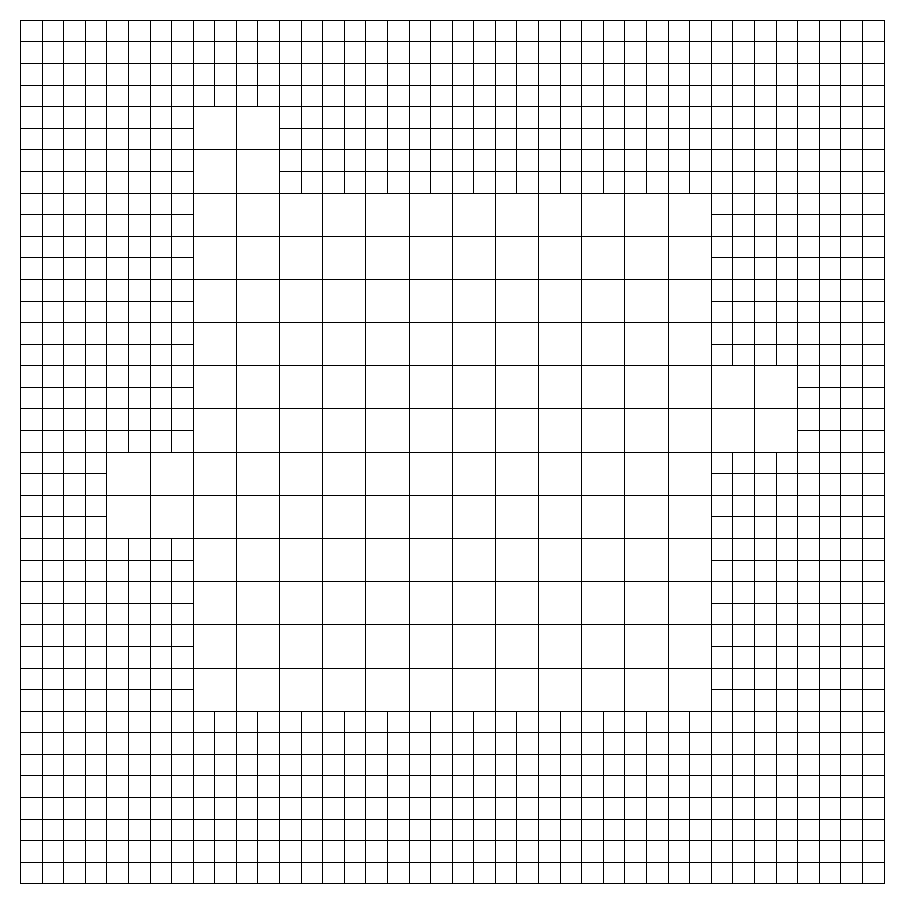
\includegraphics[height=.22\textheight]{figures/grid1} & & \\
          & & 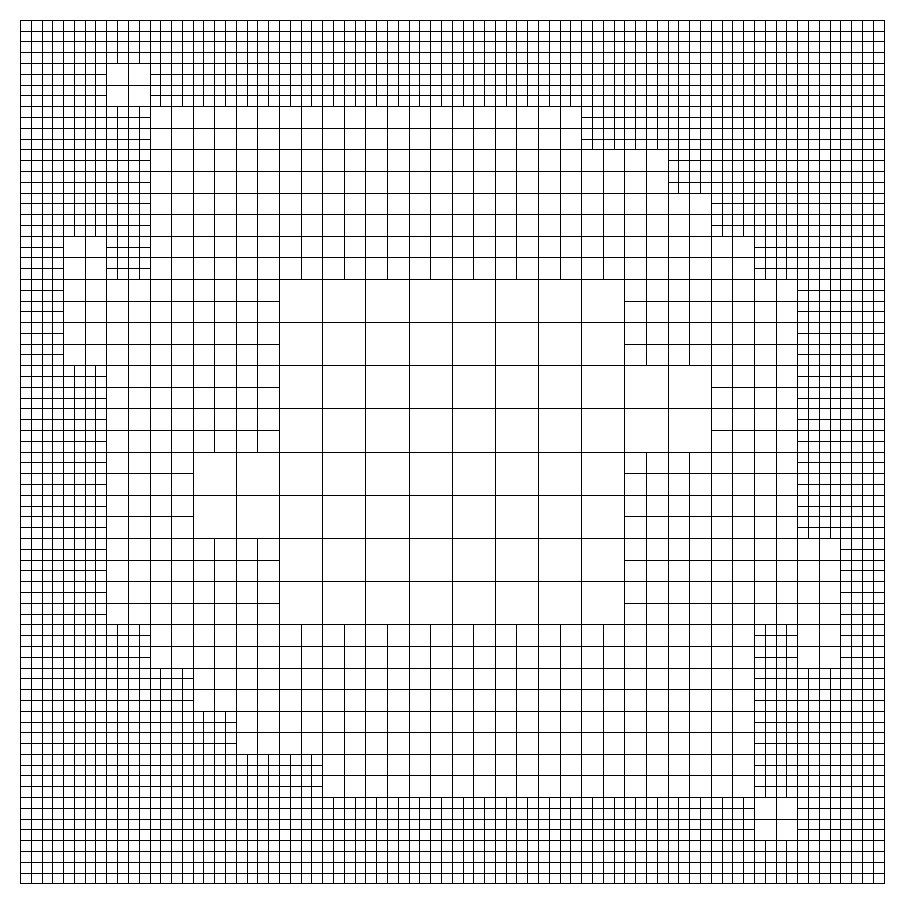
\includegraphics[height=.22\textheight]{figures/grid2} & Finish \\
          & & & 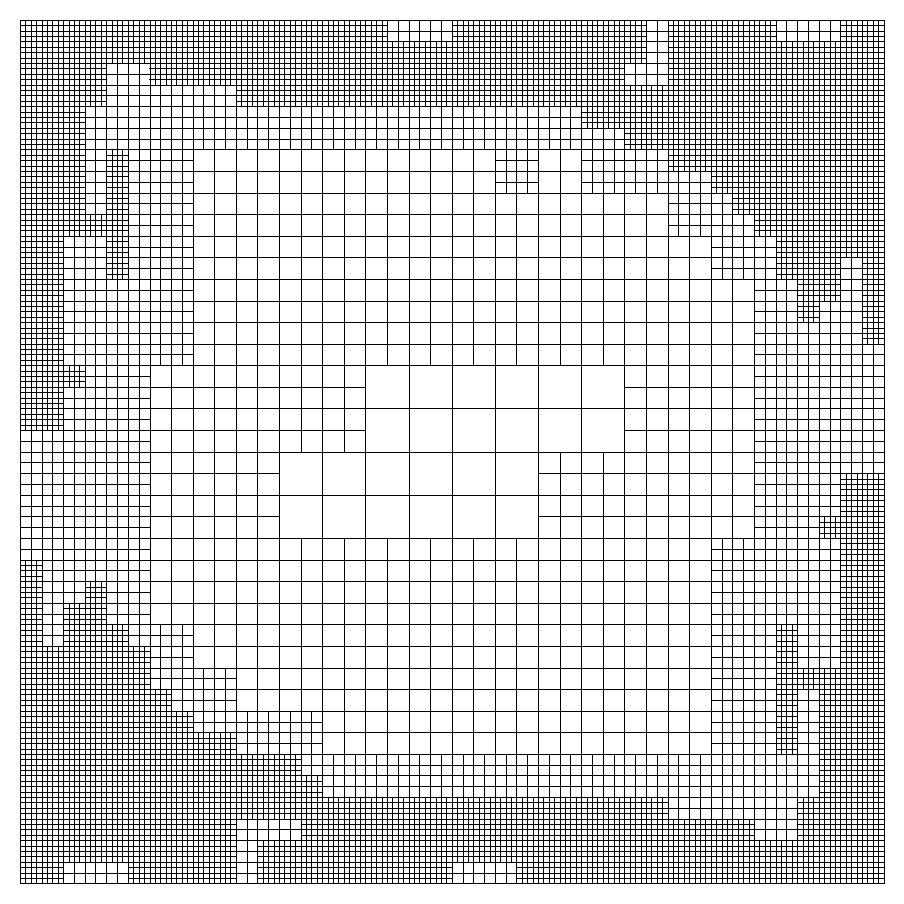
\includegraphics[height=.22\textheight]{figures/grid3} \\
        \end{tabular}
      \end{center}
    }
 
    \FirstOnly{}{
      \vspace{-.5in}
      \centerline{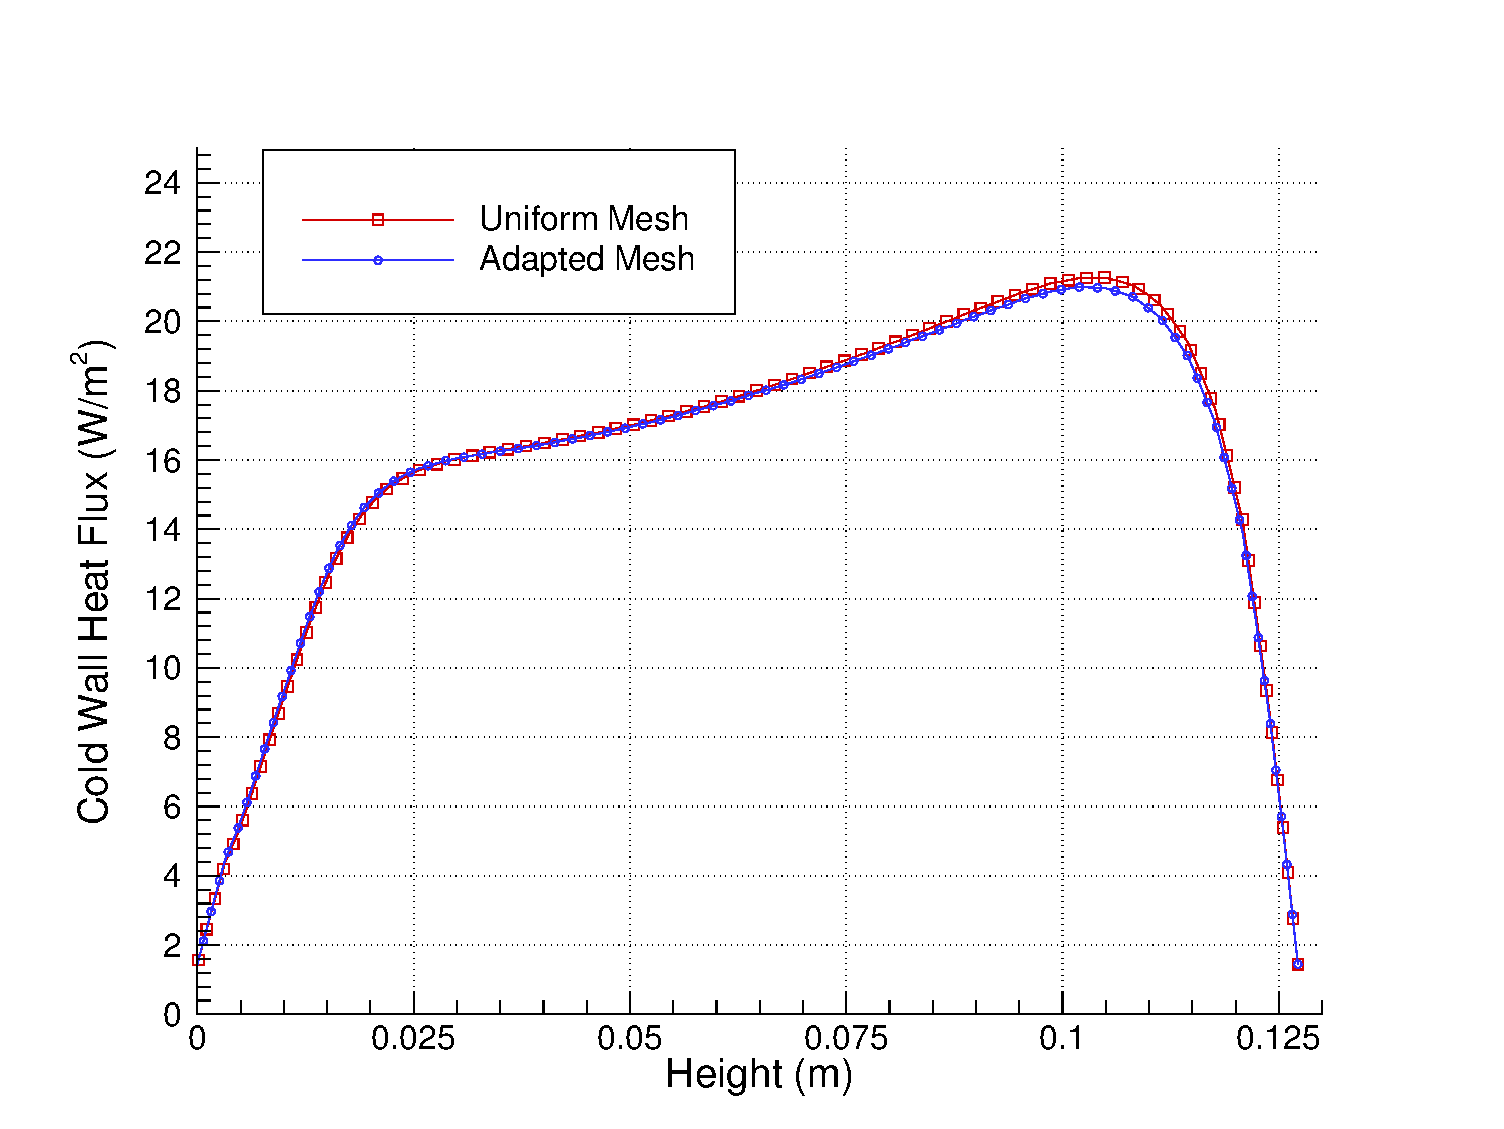
\includegraphics[width=.9\textwidth]{figures/qwall}}
    }
    \FirstOnly{}{
      \emph{* Results presented at the AMFLOW conference in Heidelberg, Germany, 2001.}
    }
  }
\end{foil}



%%%%%%%%%%%%%%%%%%%%%%%%%%%%%%%%%%%%%%%%%%%%%%%%%%%%%%%%%%%%%%%%%%%%%%%%%%%%%%%
\begin{foil}{Subgrid Strategies}
  \stepwise*{
    \FirstOnly{}{
      \begin{itemize}
        \item ``Subgrids'' can be used to locally enhance the quality of an approximate solution
	  \begin{itemize}
	    \item ``Windowing'' has often been used in commercial computer codes to focus on features of interest
	  \end{itemize}
	\item May be applicable in convection-dominated processes to stabilize the solution
      \end{itemize}
    }
    \FirstOnly{}{
      \centerline{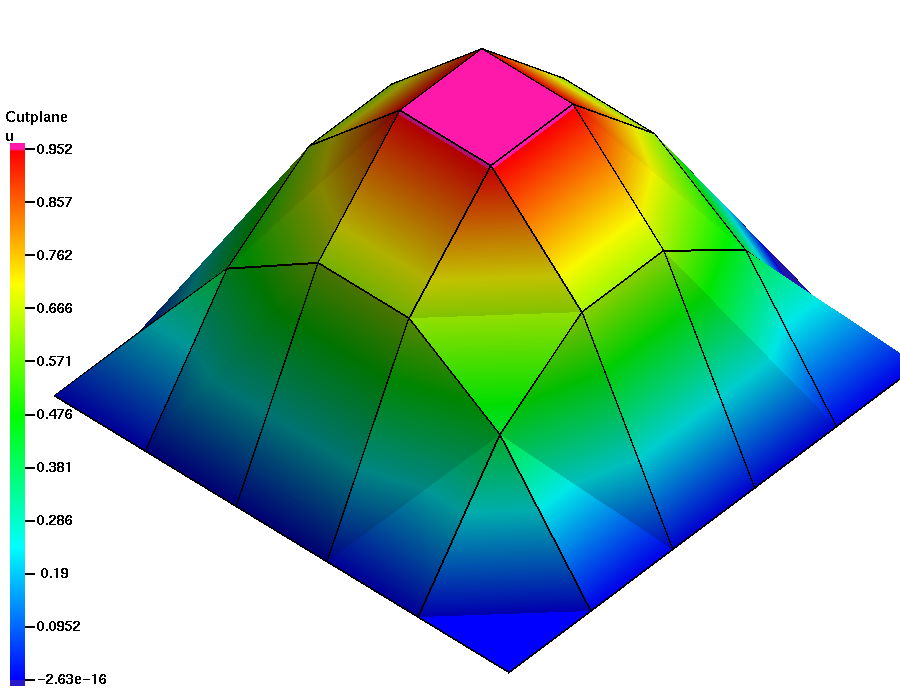
\includegraphics[width=.8\textwidth]{figures/00}}
    }
    \FirstOnly{}{
      \centerline{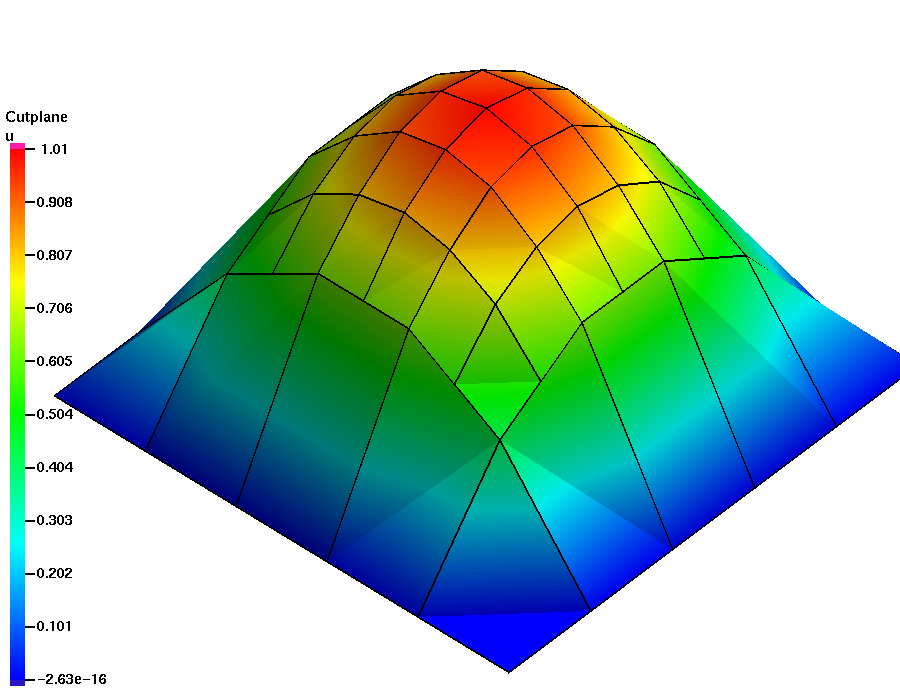
\includegraphics[width=.8\textwidth]{figures/01}}
    }
    \FirstOnly{}{
      \centerline{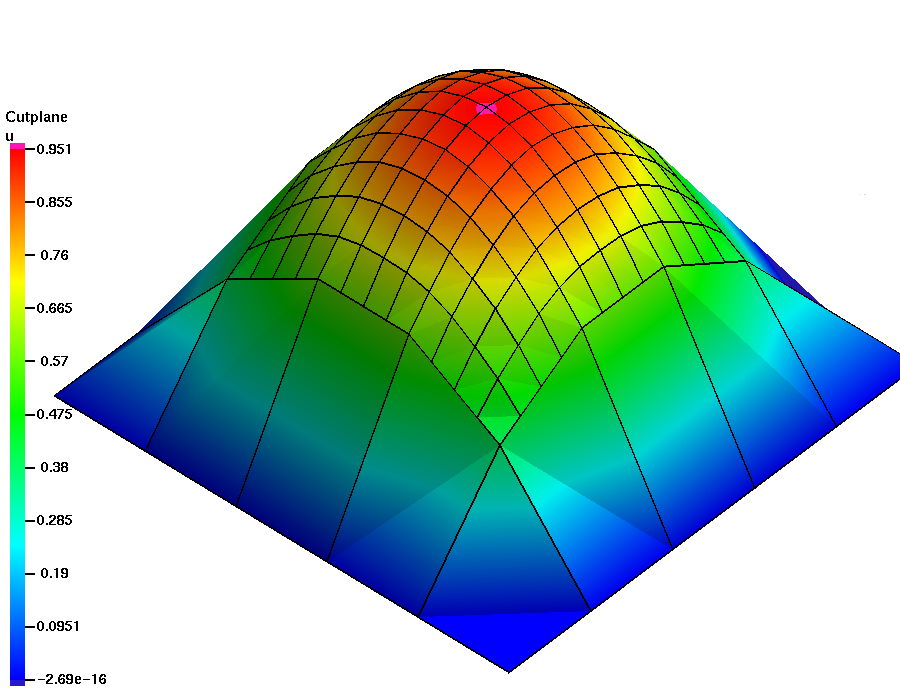
\includegraphics[width=.8\textwidth]{figures/02}}
    }
    \FirstOnly{}{
      \centerline{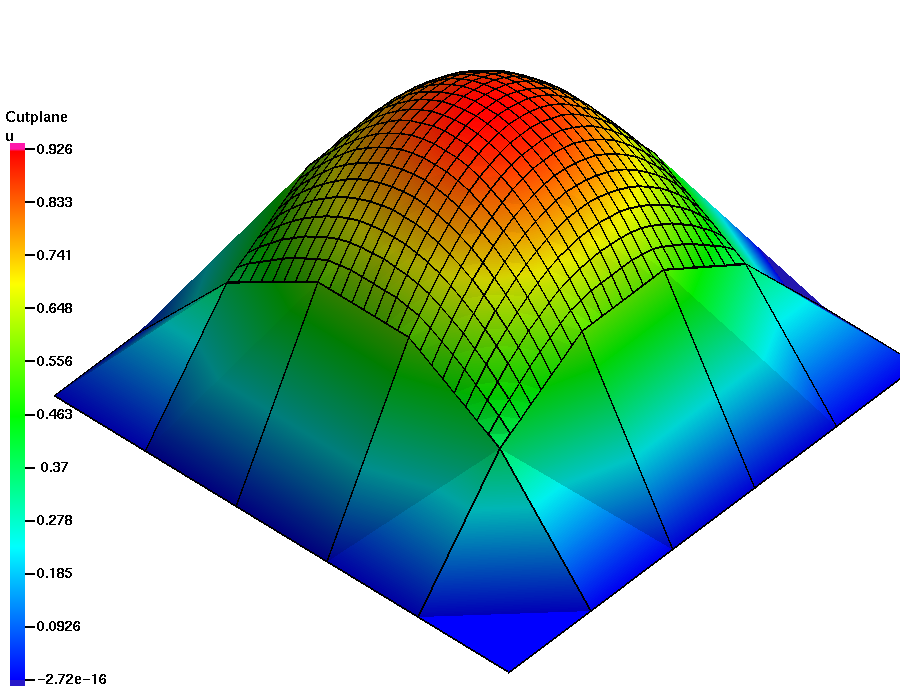
\includegraphics[width=.8\textwidth]{figures/03}}
    }
  }
\end{foil}



%%%%%%%%%%%%%%%%%%%%%%%%%%%%%%%%%%%%%%%%%%%%%%%%%%%%%%%%%%%%%%%%%%%%%%%%%%%%%%%
\begin{foil}{Adaptive Mesh Refinement}
  \begin{itemize}
    \item Adaptive Mesh Refinement (AMR) is widely recognized as a key
          technology for the efficient simulation of processes with localized and/or transient features.
    \item Many research-type AMR codes, not much support in commercial codes.
    \item Most AMR codes are serial.  Efficient AMR in 3D on parallel architectures is \emph{not trivial}.
    \item The \libMesh library has been developed to address these issues.
  \end{itemize}
\end{foil}



%%%%%%%%%%%%%%%%%%%%%%%%%%%%%%%%%%%%%%%%%%%%%%%%%%%%%%%%%%%%%%%%%%%%%%%%%%%%%%%
\begin{foil}{libMesh -- Motivation}
  \begin{itemize}
    \tightlist
  \item There are currently software libraries that address \emph{some}
        of the requirements of parallel, adaptive finite element simulations
  \item No comprehensive framework (yet) to tie these tools together
  \item No libraries with AMR support for parallel FE simulations on hybrid grids
  \item Goal:
      \begin{itemize}
      \item Provide a software framework for parallel FE simulations with AMR
      \item Support for general, unstructured meshes
      \item Use high-quality, existing software when available
      \item Create an extensive \& extensible set of tools with which applications can be easily built
      \end{itemize}
    \item The \libMesh project was started in March 2002 to meet these goals
  \end{itemize}
\end{foil}



%%%%%%%%%%%%%%%%%%%%%%%%%%%%%%%%%%%%%%%%%%%%%%%%%%%%%%%%%%%%%%%%%%%%%%%%%%%%%%%
\begin{foil}[-.25in]{libMesh -- Overview}
  \begin{itemize}
    \tightlist
    \item A C++ class library
      \begin{itemize}
        \item Highly Object-Oriented
        \item Makes extensive use of the C++ Standard Library
      \end{itemize}
    \item Open Source project, distributed under the LGPL license
    \item Runs on many platforms with native compilers:
      \begin{itemize}
        \item Linux (Intel \& Alpha)
        \item Windows (via Cygwin)
        \item IBM AIX
        \item HP-UX
        \item SGI IRIX 6.5
      \end{itemize}
    \item Under active development at:
      \begin{itemize}
        \item \href{http://cfdlab.ae.utexas.edu}{CFDLab}, The University of Texas
        \item \href{http://www.mum.tu-harburg.de/english}{Mechanics and Ocean Engineering Department},
                    Technische Universit\"{a}t Hamburg-Harburg
      \end{itemize}
  \end{itemize}
\end{foil}



%%%%%%%%%%%%%%%%%%%%%%%%%%%%%%%%%%%%%%%%%%%%%%%%%%%%%%%%%%%%%%%%%%%%%%%%%%%%%%%
\begin{foil}[-.25in]{libMesh -- Examples}
  \stepwise*{    
    \FirstOnly{}{
      \begin{center}
      	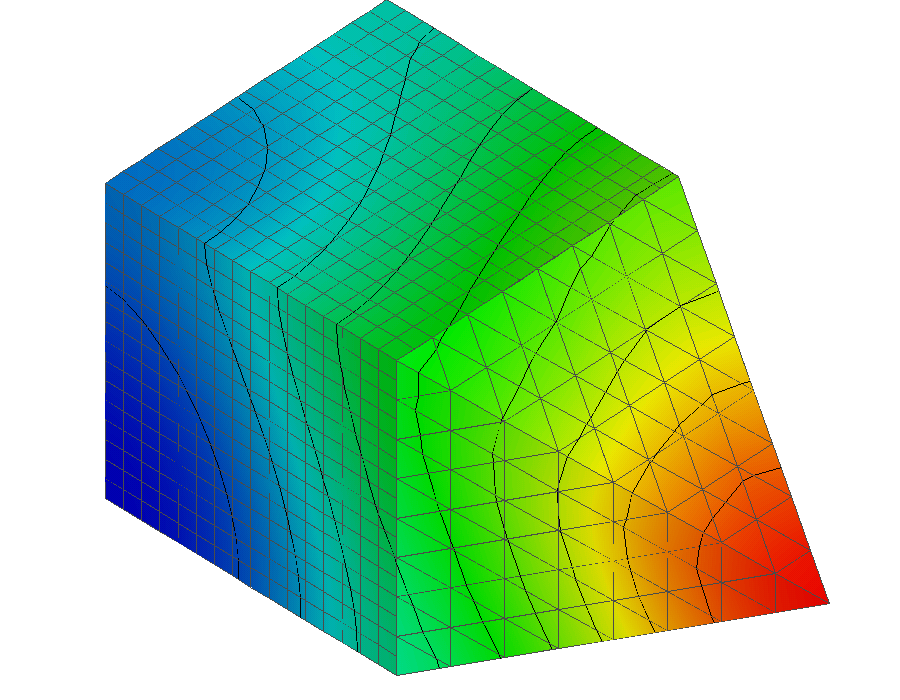
\includegraphics[width=.7\textwidth]{figures/pointy_v}
	
	3D hybrid mesh adaptively refined
      \end{center}
    }
    \FirstOnly{}{
      \centerline{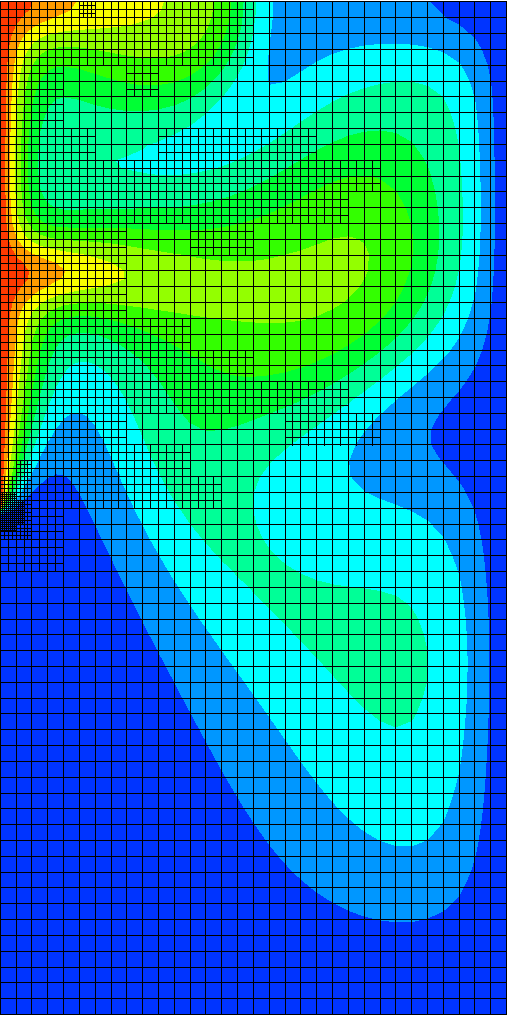
\includegraphics[angle=270,width=\textwidth]{figures/elder_amr}}
      \footnotesize
      \href{movies/elder_mesh.avi}{mesh}, \href{movies/elder_soln.avi}{solution}
      \normalsize
    }
  }
\end{foil}  



%%%%%%%%%%%%%%%%%%%%%%%%%%%%%%%%%%%%%%%%%%%%%%%%%%%%%%%%%%%%%%%%%%%%%%%%%%%%%%%
\begin{foil}{Phenomenological Studies}
  \begin{itemize}
    \item Compressible Flows
      \begin{itemize}
	\item AMR for compressible flows
	\item Shock-ramp
	\item Inlet
      \end{itemize}
  \end{itemize}
\end{foil}  



%%%%%%%%%%%%%%%%%%%%%%%%%%%%%%%%%%%%%%%%%%%%%%%%%%%%%%%%%%%%%%%%%%%%%%%%%%%%%%%
\begin{foil}[-.25in]{Compressible Flows}
  \stepwise*{
    \FirstOnly{}{
      \begin{center}
        \begin{tabular}{cc}
          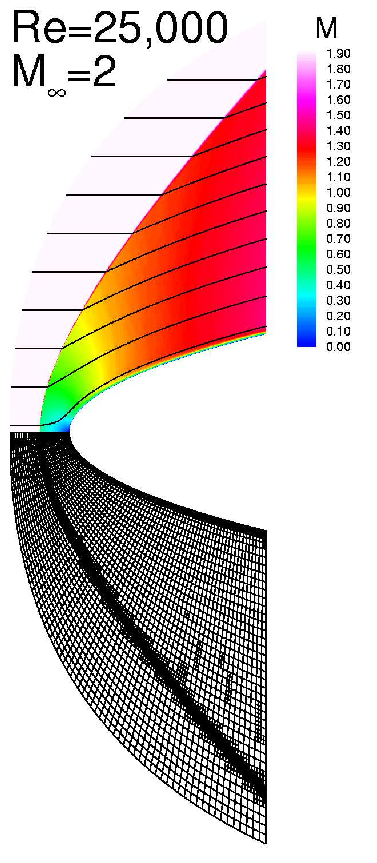
\includegraphics[height=.85\textheight]{figures/bullet_M2} &
          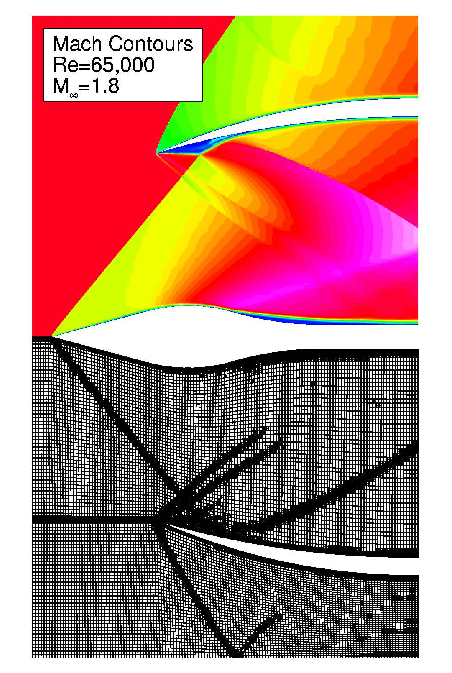
\includegraphics[height=.85\textheight]{figures/inlet} \\
        \end{tabular}
      \end{center}
    }
    \FirstOnly{}{
      \centerline{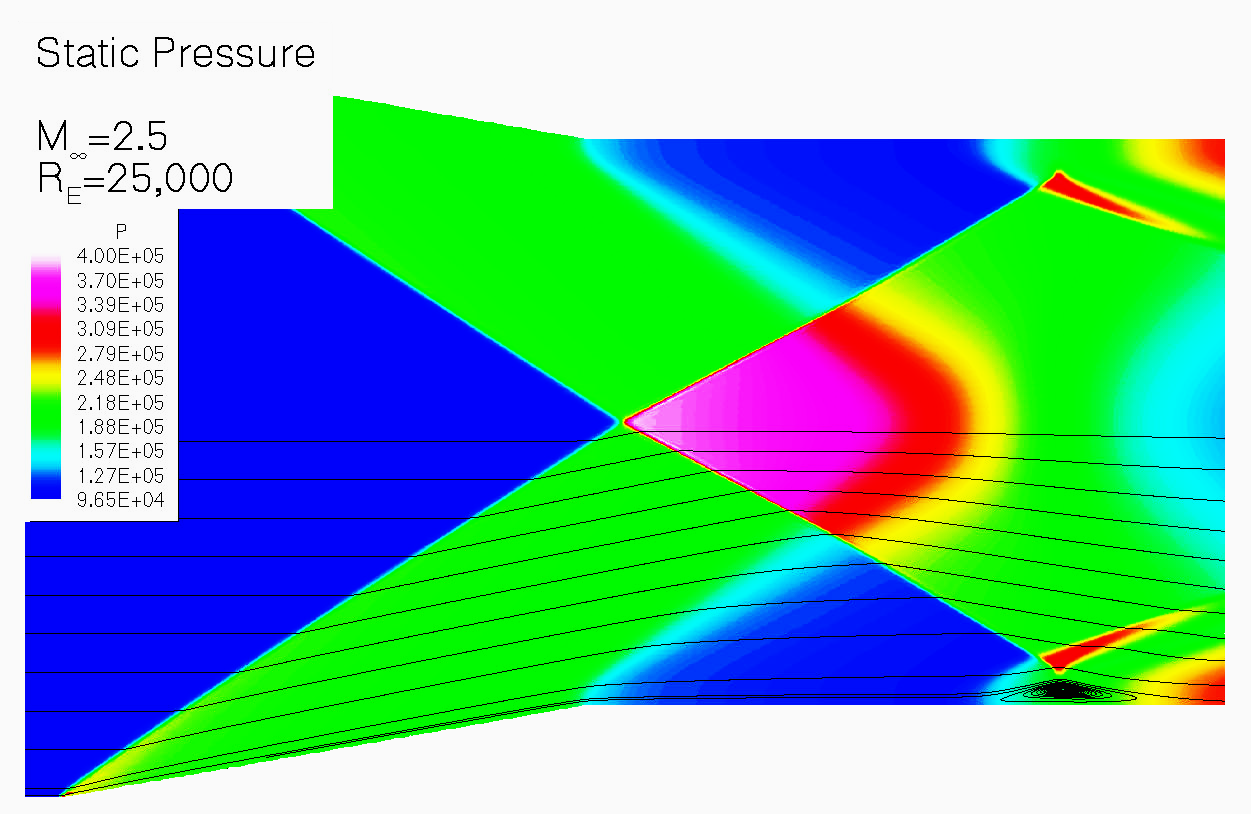
\includegraphics[width=\textwidth]{figures/p}}
    }
    \FirstOnly{}{
      \centerline{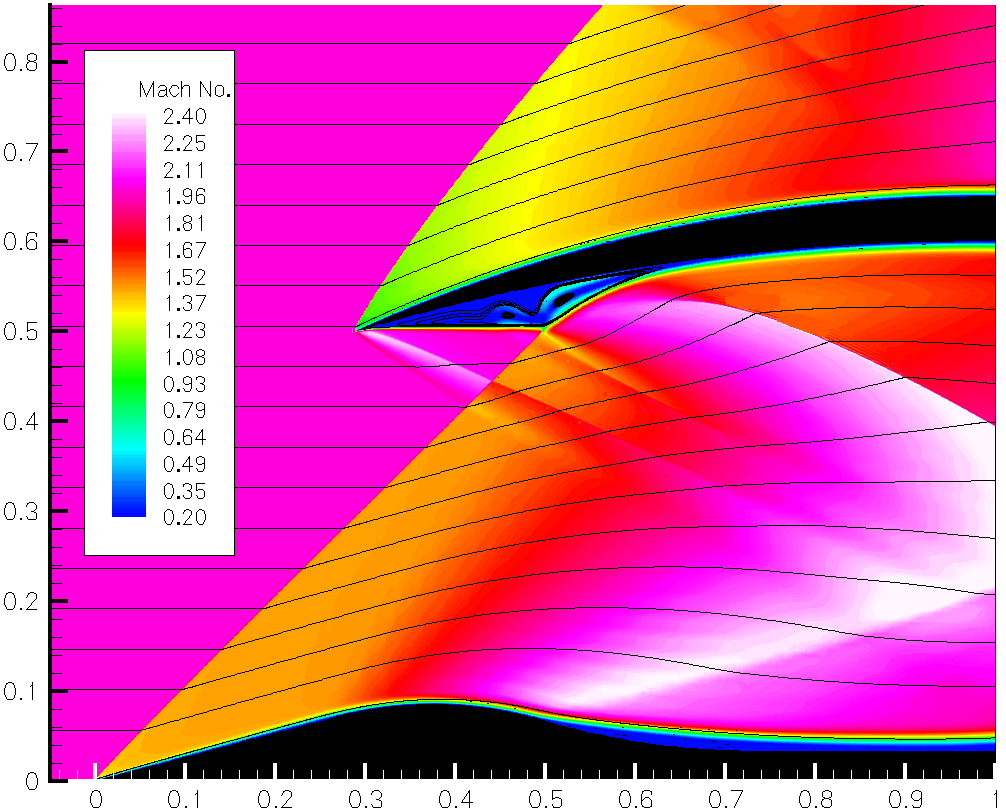
\includegraphics[height=.85\textheight]{figures/inlet_mach2_mach}}
    }
%%     \FirstOnly{}{
%%       \centerline{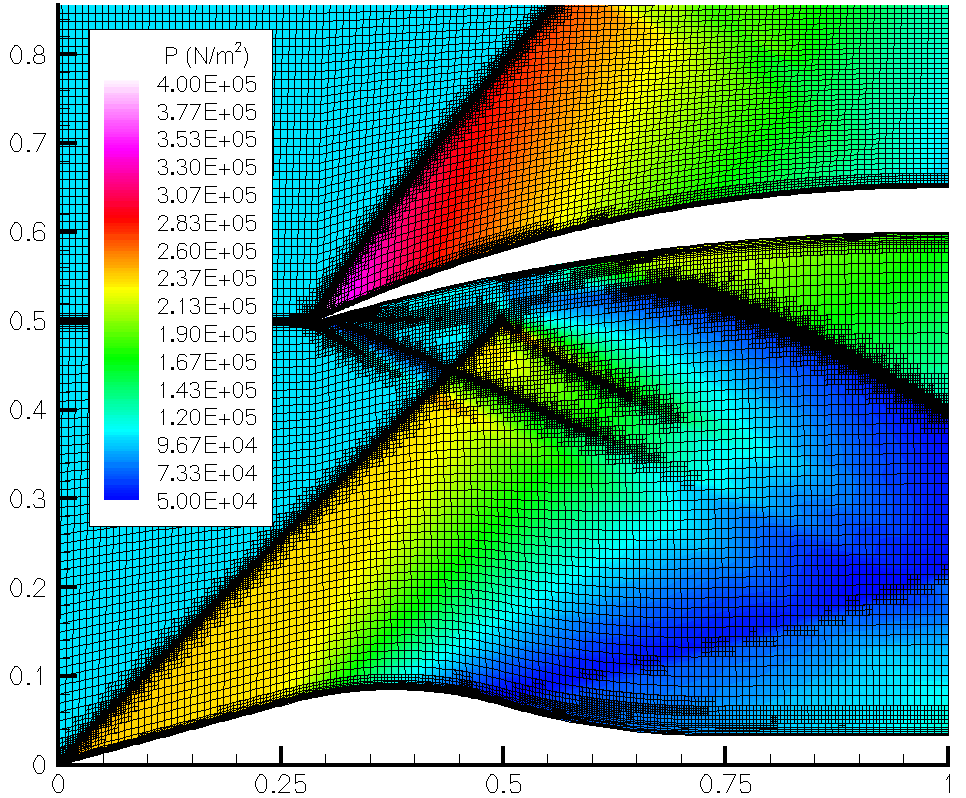
\includegraphics[height=.85\textheight]{figures/inlet_mach2_P_grid}}
%%     }
    \FirstOnly{}{
      \emph{* Results to be published in the Journal of Computational and Applied Mathematics}
    }
  }
\end{foil}



%%%%%%%%%%%%%%%%%%%%%%%%%%%%%%%%%%%%%%%%%%%%%%%%%%%%%%%%%%%%%%%%%%%%%%%%%%%%%%%
\begin{foil}{Roadmap}
  \stepwise*{
    \FirstOnly{}{
      \begin{itemize}
	\tightlist
	\item Monotonicity/Positivity
	  \begin{itemize}
	    \item Finish paper/report considering 2D extension
	  \end{itemize}
	\item Nested Grids
	  \begin{itemize}
	    \item 3D natural convection in parallel
	    \item Steady compressible flows
	  \end{itemize}
	\item Subgrid Strategies
	  \begin{itemize}
	    \item Convection-dominated processes
	    \item More analysis 
	  \end{itemize}
	\item AMR Research
	  \begin{itemize}
	    \item Parallel data structures
	  \end{itemize}
	\item Phenomenological studies
	  \begin{itemize}
	    \item Transient 2D compressible flow applications
	    \item Possible 3D extensions
	  \end{itemize}
      \end{itemize}
    }
    \FirstOnly{}{
      \begin{itemize}
	\item I will begin working at NASA Johnson Space Center immediately following the 2003 Fall semester
	\item I will be involved in hypersonic aerothermodynamics
	\item NASA is giving me flexibility to finish my dissertation
	  \begin{itemize}
	    \item Travel days
	    \item Tuition assistance
	  \end{itemize}
      \end{itemize}
    }
  }
\end{foil}






\end{document}


%% Local Variables:
%% mode: latex
%% End:
 